\chapter{Container und VMs}

Container werden oft als “lightweight VMs” bezeichnet, da beide Technologien das Ziel haben, eine Applikation in einer isolierten Umgebung laufen zu lassen, um die Applikationen portabel zu halten und Schäden am Host-System zu verhindern \cite{docker:cvsvm}.
Und doch haben beide Technologien wenig gemeinsam. Während im Falle der virtuellen Maschinen ein komplettes System mit Hardware, Betriebssystem und Applikation simuliert wird, reicht es für das Ausführen einer Applikation in einem Container die nötigen Bibliotheken mitzuliefern.
Ein weiterer großer Unterschied ist, dass VMs einen Zustand haben. Sie repräsentiert ein komplettes System mit Prozessen und Daten, das woanders wieder in genau diesem Zustand weiterlaufen kann. Container hingegen sind meist zustandslos.\\

\begin{figure}[!ht]
  \centering
  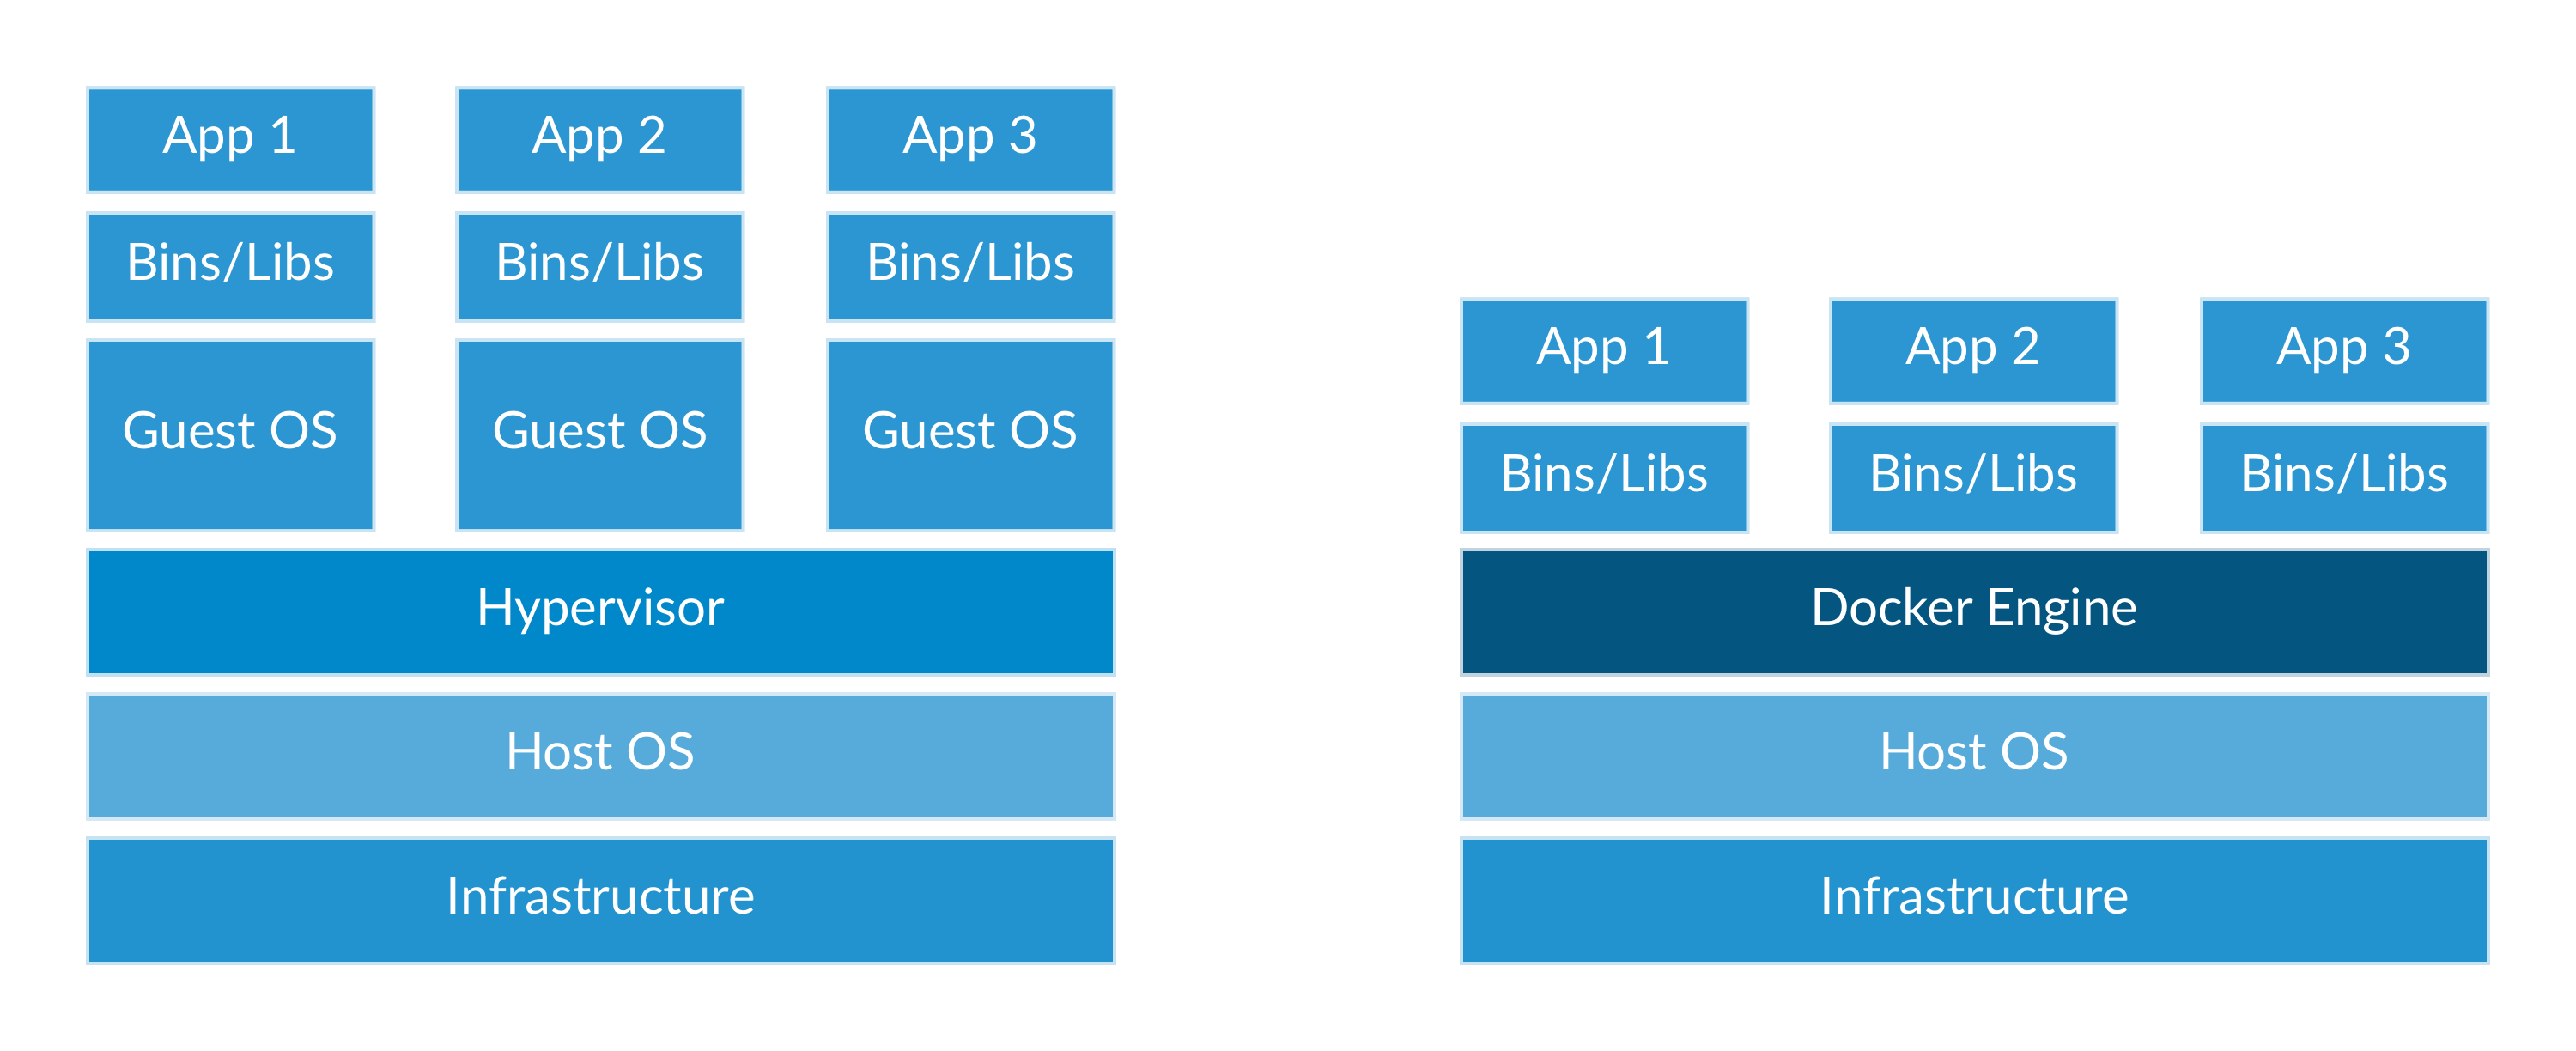
\includegraphics[width=1\textwidth]{images/6-container-vm.png}
  \caption{Verschiedene VMs und Container auf einem Host-System im Vergleich \cite{docker}}
\end{figure}

\noindent Es gibt keine Regeln dafür, wann eine Applikation innerhalb eines Containers und wann sie innerhalb einer VM laufen sollte. Das kommt auf die Applikation an und muss von Fall zu Fall betrachtet werden. Bei einer älteren monolithischen Webanwendung, also einer, die alle nötigen Services und Komponenten, wie Frontend, Backend und die Datenbanken, beinhaltet, macht es Sinn diese weiter in einer virtuellen Maschine zu starten. Besteht die Anwendung aus vielen kleinen spezialisierten Microservices, macht es Sinn diese in einzelnen Containern zu starten. Grundsätzlich schließen sich beide Technologien aber auch nicht aus, da Container auf allen Host-Systemen gestartet werden können, die auf dem gleichen Kernel aufbauen - also auch virtuellen Maschinen. Sollen Anwendungen die in Containern laufen beispielsweise mit älteren, in VMs laufenden Anwendungen zusammenarbeiten, bei denen klar ist, dass diese nicht noch einmal überarbeitet werden sollen, können diese einfach mit auf der VM gestartet werden. So können die Vorteile beider Technologien miteinander kombiniert werden. \cite{docker:cavm}. Wer vor allem auf Sicherheit wert legt, sollte wahrscheinlich erst einmal weiter auf virtuelle Maschinen setzen, da es bei diesen für Prozesse nicht möglich ist aus der Isolation auszubrechen. Bei Containern hingegen handelt es sich um eine vergleichsweise junge Technologie, bei der durchaus noch Sicherheitslücken auftreten könnten.\\

\begin{figure}[!ht]
  \centering
  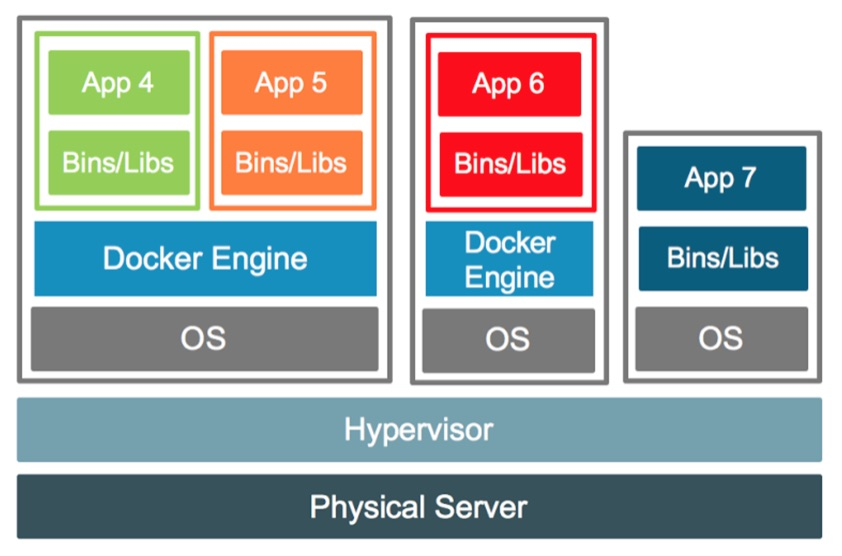
\includegraphics[width=0.6\textwidth]{images/7-container-vm-combined.jpg}
  \caption{VMs und Docker Container kombinier \cite{docker:cavm}}
\end{figure}
